\documentclass[12pt, titlepage]{article}

\usepackage{graphicx}
\usepackage{wrapfig}
\usepackage{hyperref}
\usepackage{siunitx}
\usepackage{amsmath}
\usepackage{enumerate}

\title{Flippin' Flingers Trebuchet Progress Report}
\author{Omar Ebrahim 110076575\\Saif Kaoud 110076323\\[10pt] Dr. John Magliaro\\
University of Windsor}

\begin{document}
    \maketitle
    \section{Summary}
    \newpage
    \tableofcontents \newpage
    \listoffigures
    \listoftables \newpage
    \section{Introduction}
    This report's mission statement is to summarize the team's progress with:
    \begin{itemize}
        \item Preliminary design sketches.
        \item Detailed CAD drawings.
        \item Numerical modeling details and range predictions.
    \end{itemize}
    The problem outline is to design and analyze the trebuchet to maximize
    projectile distance and accuracy.\\[10pt]
    The trebuchet is designed for maximum distance through general
    plane motion.\footnote{Hibbeler, 2015}It is also designed for maximum 
    accuracy through string measure.\footnote{Rhoten, 2021}\\[10pt]
    To maximize distance, the velocity of the projectile is considered, as
    distance and velocity are proportional. Increasing the counterweight 
    fall distance can boost the projectile's velocity.\footnote{Siano, 2001}
    Increasing the counterweight-to-launch distance increases the velocity 
    of the projectile.\footnote{Denny, 2005}\\[10pt]
    Lastly, adjusting the trebuchet firing angle to 
    45 degrees achieves the maximum projectile distance.\footnote{Connel, 2001}
    \newpage
    \section{Trebuchet}
    \subsection{Sketch}
    Based on the provided information, the team chose to build a Floating Arm 
    Trebuchet, which is recognized for its unique feature of an axle allowing 
    unrestricted movement on the throwing arm. As a result, the trebuchet 
    exhibits general plane motion. The sketch is shown in Figure \ref{sketch}.\\[10pt]
    The frame of a trebuchet serves as the structural backbone that supports 
    and stabilizes the entire machine, and the arm is connected to the frame
    with wooden wheels.\\[10pt]
    The counterweight is released once the guide chute is triggered.
    When the counterweight is released, it falls, causing the throwing arm 
    to rotate rapidly around the axle. As the arm swings, the projectile 
    is released from the sling.
    \begin{figure}[t]                                  
    \centering
    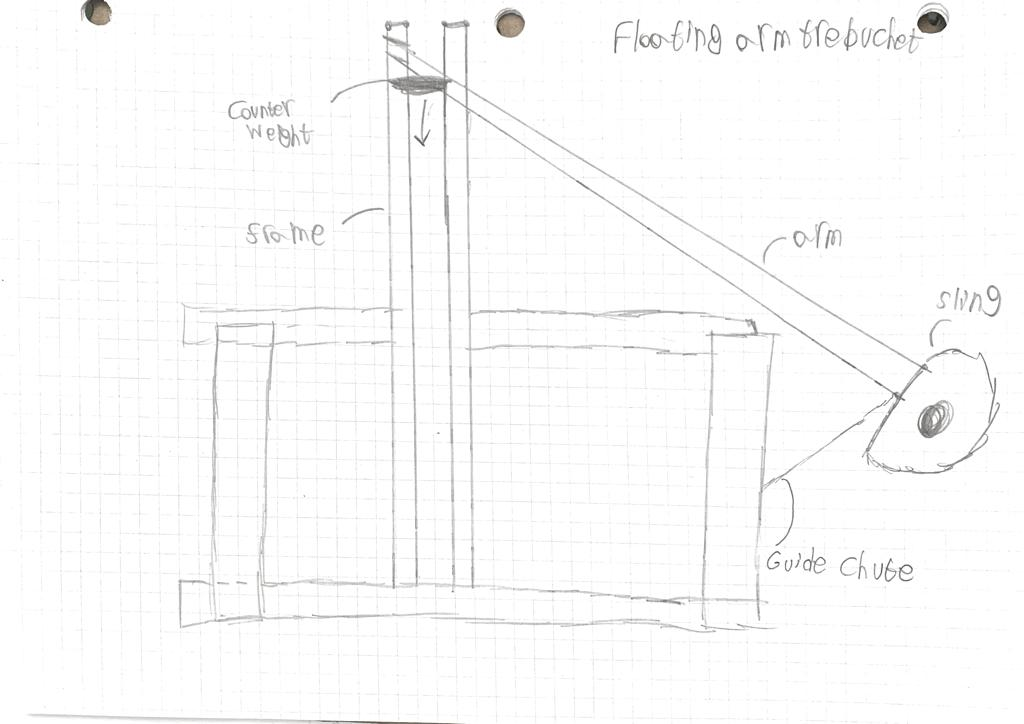
\includegraphics[width=0.8\textwidth]{sketch.jpeg}
    \caption{Floating Arm Trebuchet sketch\label{sketch}}
    \end{figure}
    \newpage
    \subsection{Design}
    l
    \newpage
    \subsection{Model}
    \newpage
    \section{Conclusions}
    The main objectives of this milestone were [complete the statement].
    The key findings are summarized as follows:
    \begin{enumerate}
        \item l
    \end{enumerate}
    \newpage
    \section{References}
        \hspace{15pt}Hibbeler, R. C. (2015). 16.5. In Engineering mechanics: Dynamics (pp. 346–348). essay, Pearson.

        Rhoten, R. P. (1999). The trebuchet: Accuracy analysis of a medieval siege engine. Volume 2: 19th Computers and Information in Engineering Conference.

        Siano, D. B. (2001). Trebuchet Mechanics. The Algorithmic Beauty of the Trebuchet.

        Denny, M. (2005). Siege engine dynamics. European journal of physics, 26(4), 561.

        James O'Connell; Dynamics of a medieval missile launcher: the trebuchet. The Physics
        Teacher 1 November 2001; 39 (8): 471–473.
    \newpage
\end{document}
